\documentclass[10pt,a4paper]{standalone}
\usepackage{amssymb}
\usepackage{amsmath}
\usepackage{bm}
\usepackage{tikz}
\usetikzlibrary{arrows.meta}
\usetikzlibrary{arrows}
\usepackage{pstricks}
\usetikzlibrary{patterns}
\usetikzlibrary{fadings}
\usetikzlibrary{shapes.geometric}


\begin{document}
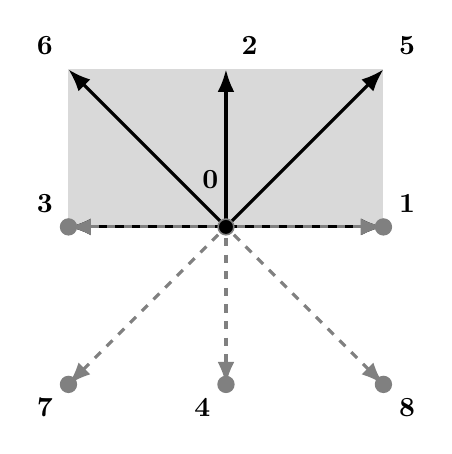
\begin{tikzpicture}[line width=0.2mm]


\fill[gray!30] (4,4) -- (8,4) -- (8,6) -- (4,6) -- cycle;



\draw[-Latex,shorten <=-2pt,solid,line width=0.4mm] (6,4) -- (8,4); %1
\draw[-Latex,shorten <=-2pt,dashed,gray,line width=0.4mm] (6,4) -- (8,4); %1
\draw[-Latex,shorten <=-2pt,solid,line width=0.4mm] (6,4) -- (4,4); %3
\draw[-Latex,shorten <=-2pt,dashed,gray,line width=0.4mm] (6,4) -- (4,4); %3
\draw[-Latex,shorten <=-2pt,solid,line width=0.4mm] (6,4) -- (6,6); %2
\draw[-Latex,shorten <=-2pt,dashed,gray,line width=0.4mm] (6,4) -- (6,2); %4
\draw[-Latex,shorten <=-2pt,solid,line width=0.4mm] (6,4) -- (8,6); %5
\draw[-Latex,shorten <=-2pt,solid,line width=0.4mm] (6,4) -- (4,6); %5
\draw[-Latex,shorten <=-2pt,dashed,gray,line width=0.4mm] (6,4) -- (4,2); %7
\draw[-Latex,shorten <=-2pt,dashed,gray,line width=0.4mm] (6,4) -- (8,2); %8


\draw (5.8,4.6)node[]{$\mathbf{0}$};
\draw (8.3,4.3)node[]{$\mathbf{1}$};
\draw (6.3,6.3)node[]{$\mathbf{2}$};
\draw (3.7,4.3)node[]{$\mathbf{3}$};
\draw (5.7,1.7)node[]{$\mathbf{4}$};
\draw (8.3,6.3)node[]{$\mathbf{5}$};
\draw (3.7,6.3)node[]{$\mathbf{6}$};
\draw (3.7,1.7)node[]{$\mathbf{7}$};
\draw (8.3,1.7)node[]{$\mathbf{8}$};

\draw[gray,fill=black] (6,4)node[]{} circle(0.1cm); %0
\draw[gray,fill=gray] (4,2)node[]{} circle(0.1cm);%7
\draw[gray,fill=gray] (6,2)node[]{} circle(0.1cm);%4
\draw[gray,fill=gray] (8,2)node[]{} circle(0.1cm);%8

\draw[gray,fill=gray] (4,4)node[]{} circle(0.1cm);%3
\draw[gray,fill=gray] (8,4)node[]{} circle(0.1cm);%1


\end{tikzpicture}
\end{document}



